\section{The Significant Degrees of the Angles**}

\subsection{\textit{[Finding the Operative Degrees]}}
First of all, fix the degree-positions of the Ascendant, MC, and the other angles. Then it is necessary to take the distance in degrees from the Ascendant to IC (moving in the order of the signs), to consider one third of that total distance to be the “operative” degrees in the configuration of the angles, and to consider the stars in these degrees, whether benefics or malefics, to be powerful. 

Consider the rest of the degrees in order up to IC, as well as the stars in them, to be “inoperative” and impropitious. The points in opposition to the Ascendant and to the other angles will fall into the same pattern with respect to operative
and inoperative degrees and the stars in <the operative degrees> will be powerful. It is therefore obvious that there will not always be 30° at an angle, but sometimes more, sometimes fewer. 

If in the Ascending and Descending signs there are fewer \textbf{/135K/} than 30 powerful degrees, then there will be more than 30° at MC and IC. 

If in the Ascending sign and its opposite there are more than 30°, then at MC and IC there will be fewer.

An example: Ascendant at \Pisces\xspace 13°, MC at \Sagittarius\xspace 22°, IC at \Gemini <22°>, Descendant at
\Virgo\xspace 13°. I take the distance from the Ascendant to IC, \textbf{/128P/} 99°. One-third of this is 33°. I count this
distance from the Ascendant and stop at \Aries\xspace 16°. These degrees and the stars in them will be powerful; the rest of the degrees from Aries 16° to IC will be inoperative. The points in opposition will have the same effect. 

Secondly I take the distance from MC to the Ascendant, 81°. One-third of this is 27°. I count this from MC and stop at \Capricorn\xspace 19°. These degrees and those in opposition to them will be operative; the rest will be inoperative. It is necessary to do likewise for other nativities in order to know whether stars are in operative or inoperative degrees.

\begin{figure}[H]
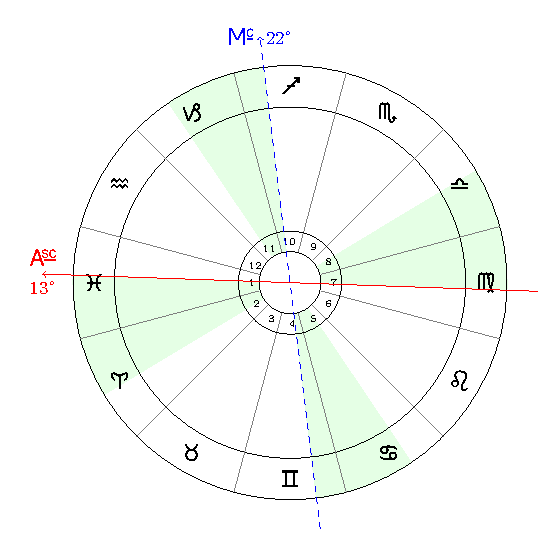
\includegraphics[width=\textwidth]{charts/3_02_operative_degrees}
\caption{Valens Book III 3.2 Operative Degrees}
\end{figure}

\subsection{\textit{[Another Method**]}}
Now to me the following method seems more scientific: take the distance from the degree in the Ascendant to IC, calculate one-third (as previously stated), then count from the Ascendant in the order of the signs, and consider these degrees and those in opposition to be powerful. Now consider the other <one-third> portion of the degrees to be average, neither completely good or bad, because this region 1) follows the Ascendant, 2) is <the III Place of> the Goddess, 3) is in opposition to <the IX Place of> the God. So then, the first third from the Ascendant will be operative and powerful, the second third will be average, the third third will be crisis-producing and bad. The stars <in these regions> will act in the same way.

It is necessary to calculate likewise from MC, and to consider the first third of the distance between angles as operative, the second third, following MC, as of average influence (thus it was called Good Daimon by the ancients), and the last third, up to the Ascendant, as afflicting and inoperative. The Places in opposition to these will have the same force. Orion expounded all this in his book.

\begin{figure}[H]
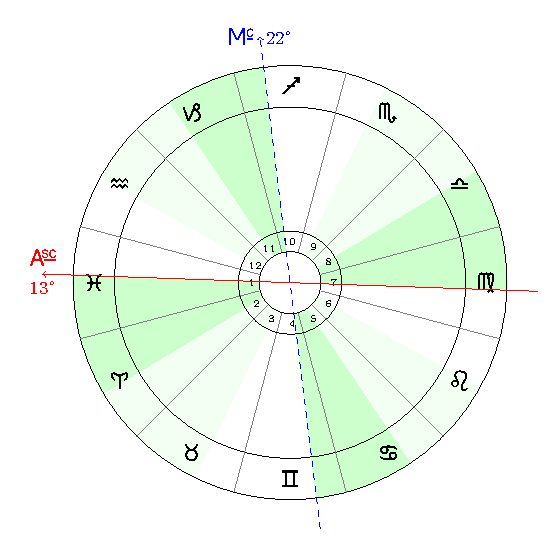
\includegraphics[width=\textwidth]{charts/3_02_Valens_opdegs}
\caption{Valens Book III 3.2 Valens Operative Degrees}
\end{figure}

\begin{mdframed}[backgroundcolor=cyan!5]
\textbf{Comment:} \hfill \\
This section is as clear as mud. It appears to equate \textsl{strength} with \textsl{quality} which makes little sense; life can throw out both types of events: powerfully good or powerfully bad. I am inclined to agree with Schmidt's contention that the 1/3's mark out ``places of greater or lesser activity on the part of the planet...places where it could properly conduct its business''. He goes on to say ``they should be used for the strength of the planet'' i.e. they are concerned with the \textsl{strength} of a planet to produce an effect and not the \textsl{quality} of the effect produced.
\end{mdframed}

\newpage